
\begin{tikzpicture}[
    every path/.style={thick,line join=round, cap=round},
]

\node[visible on=<1>] (plat) at (0,0) {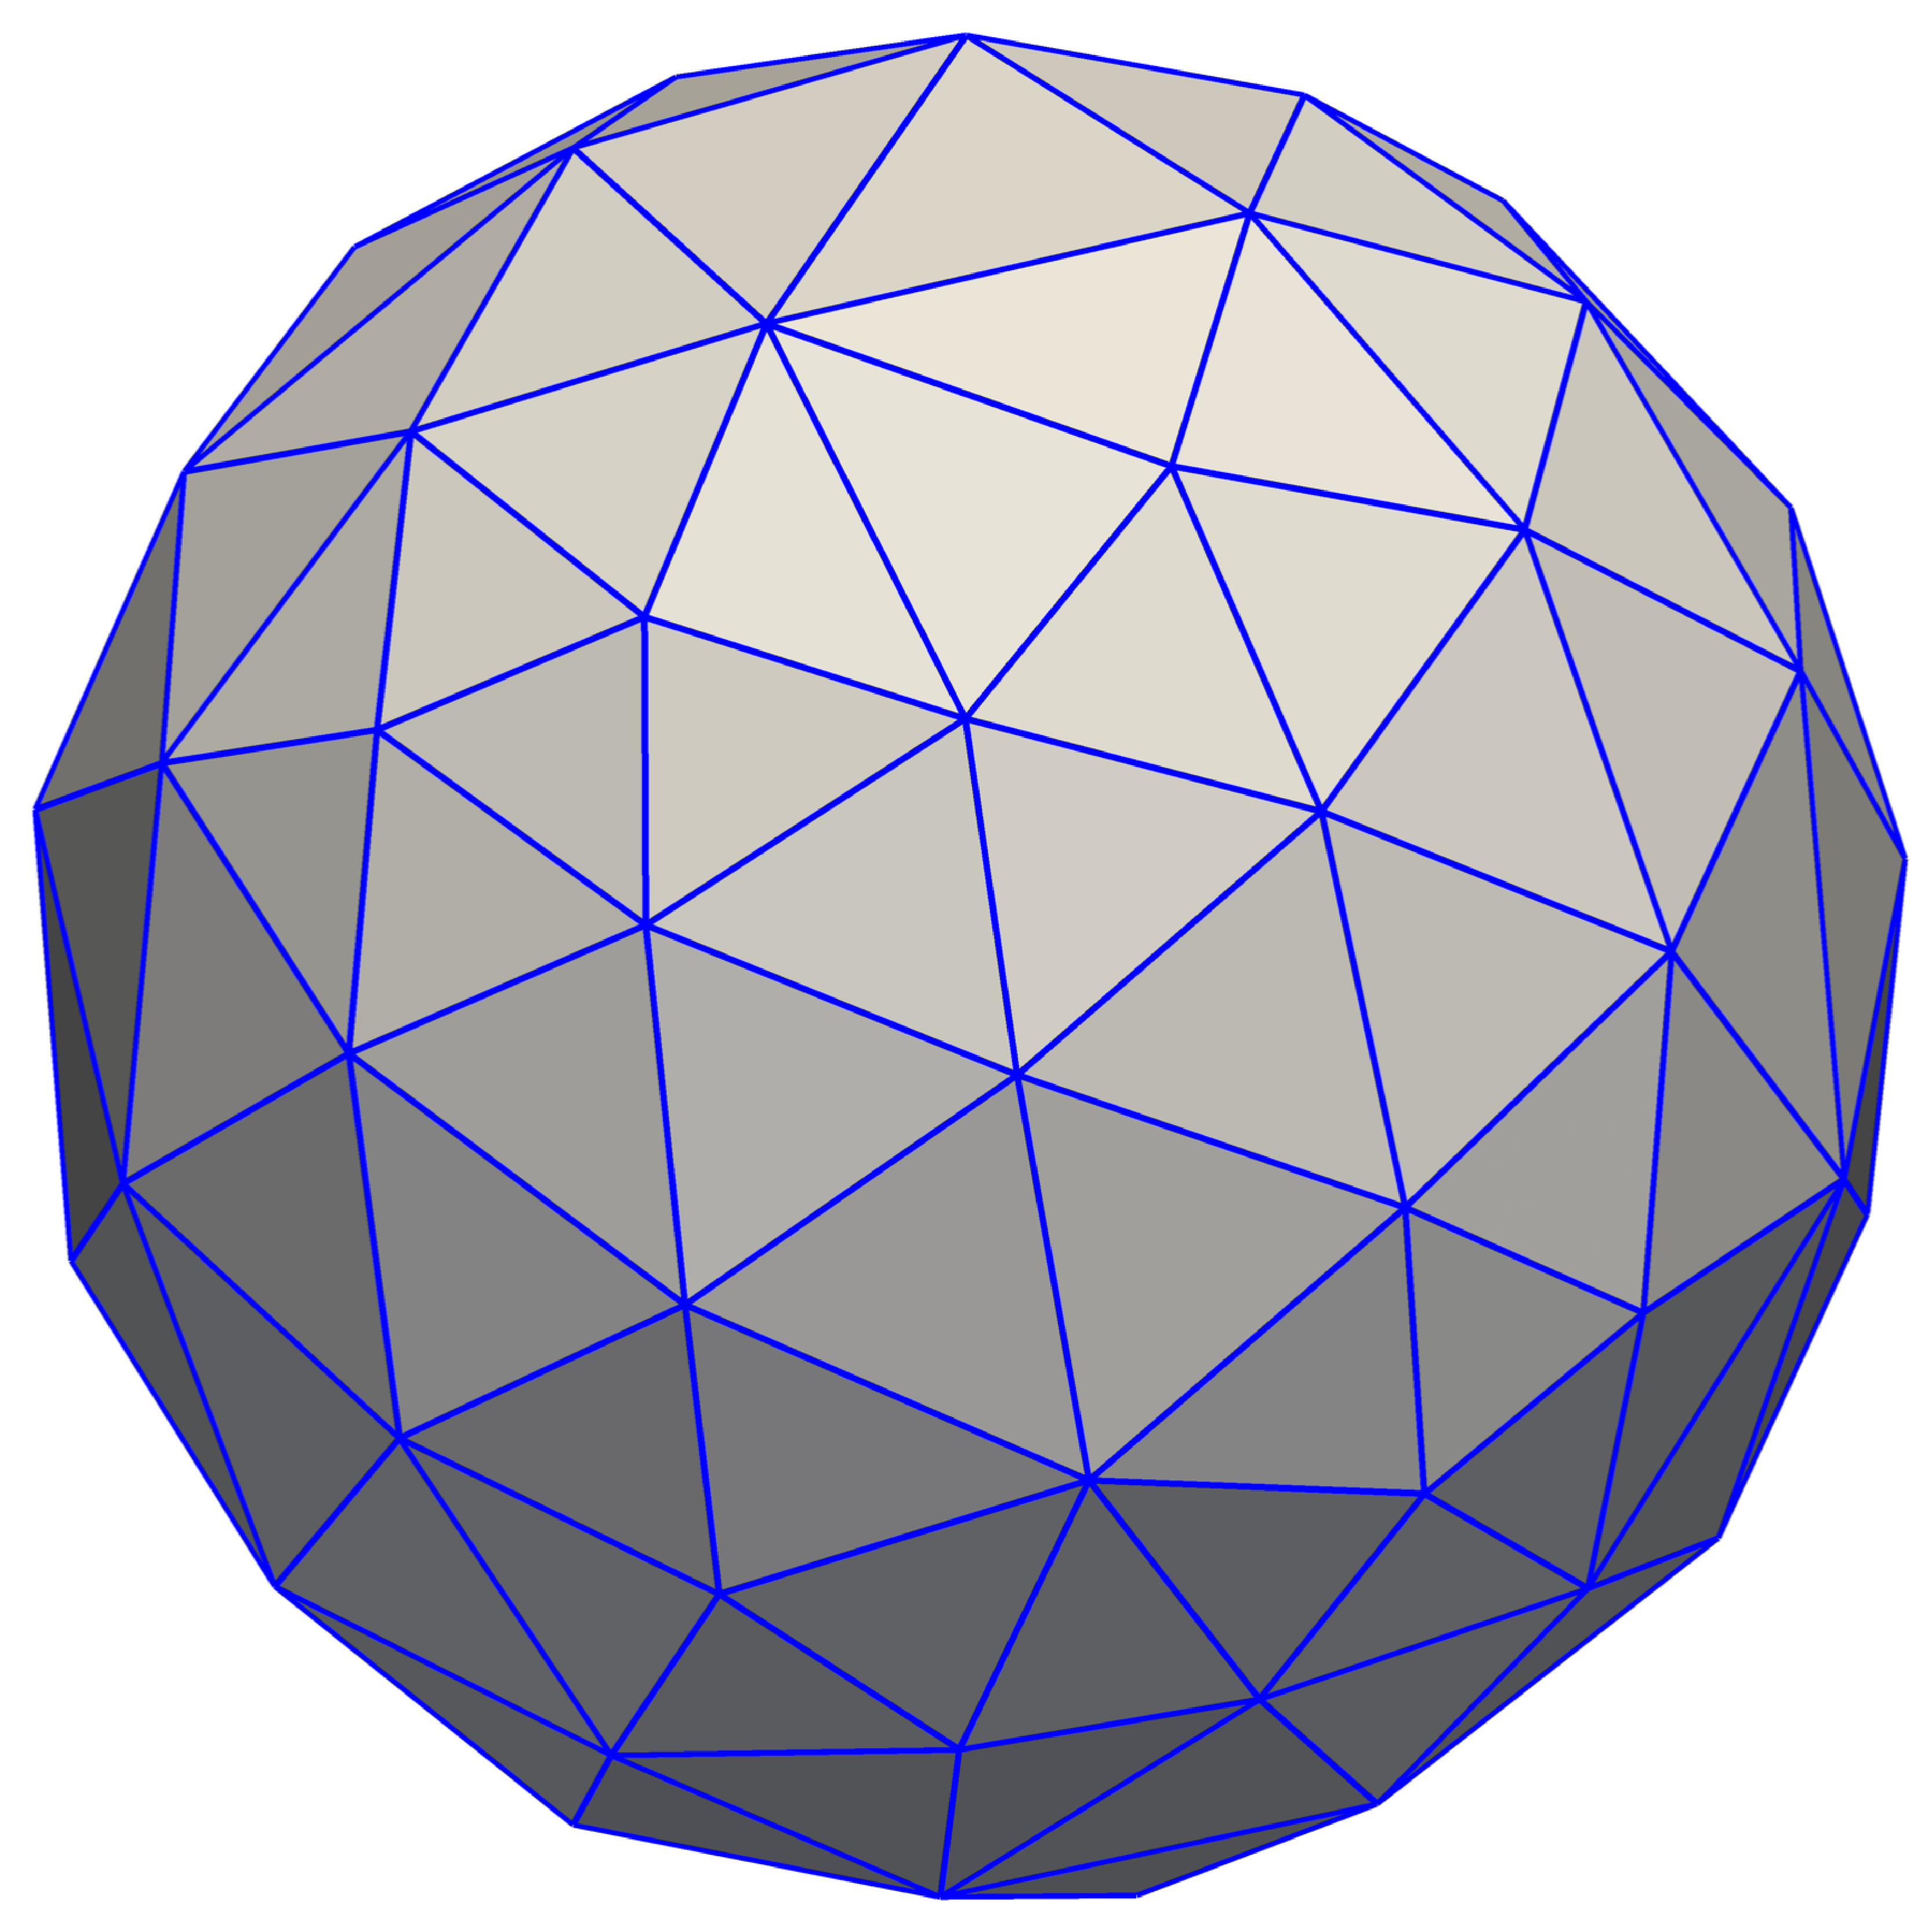
\includegraphics[width=0.6\textwidth]{img/sphere_primal.pdf}};
\node[visible on=<2>] (plat) at (0,0) {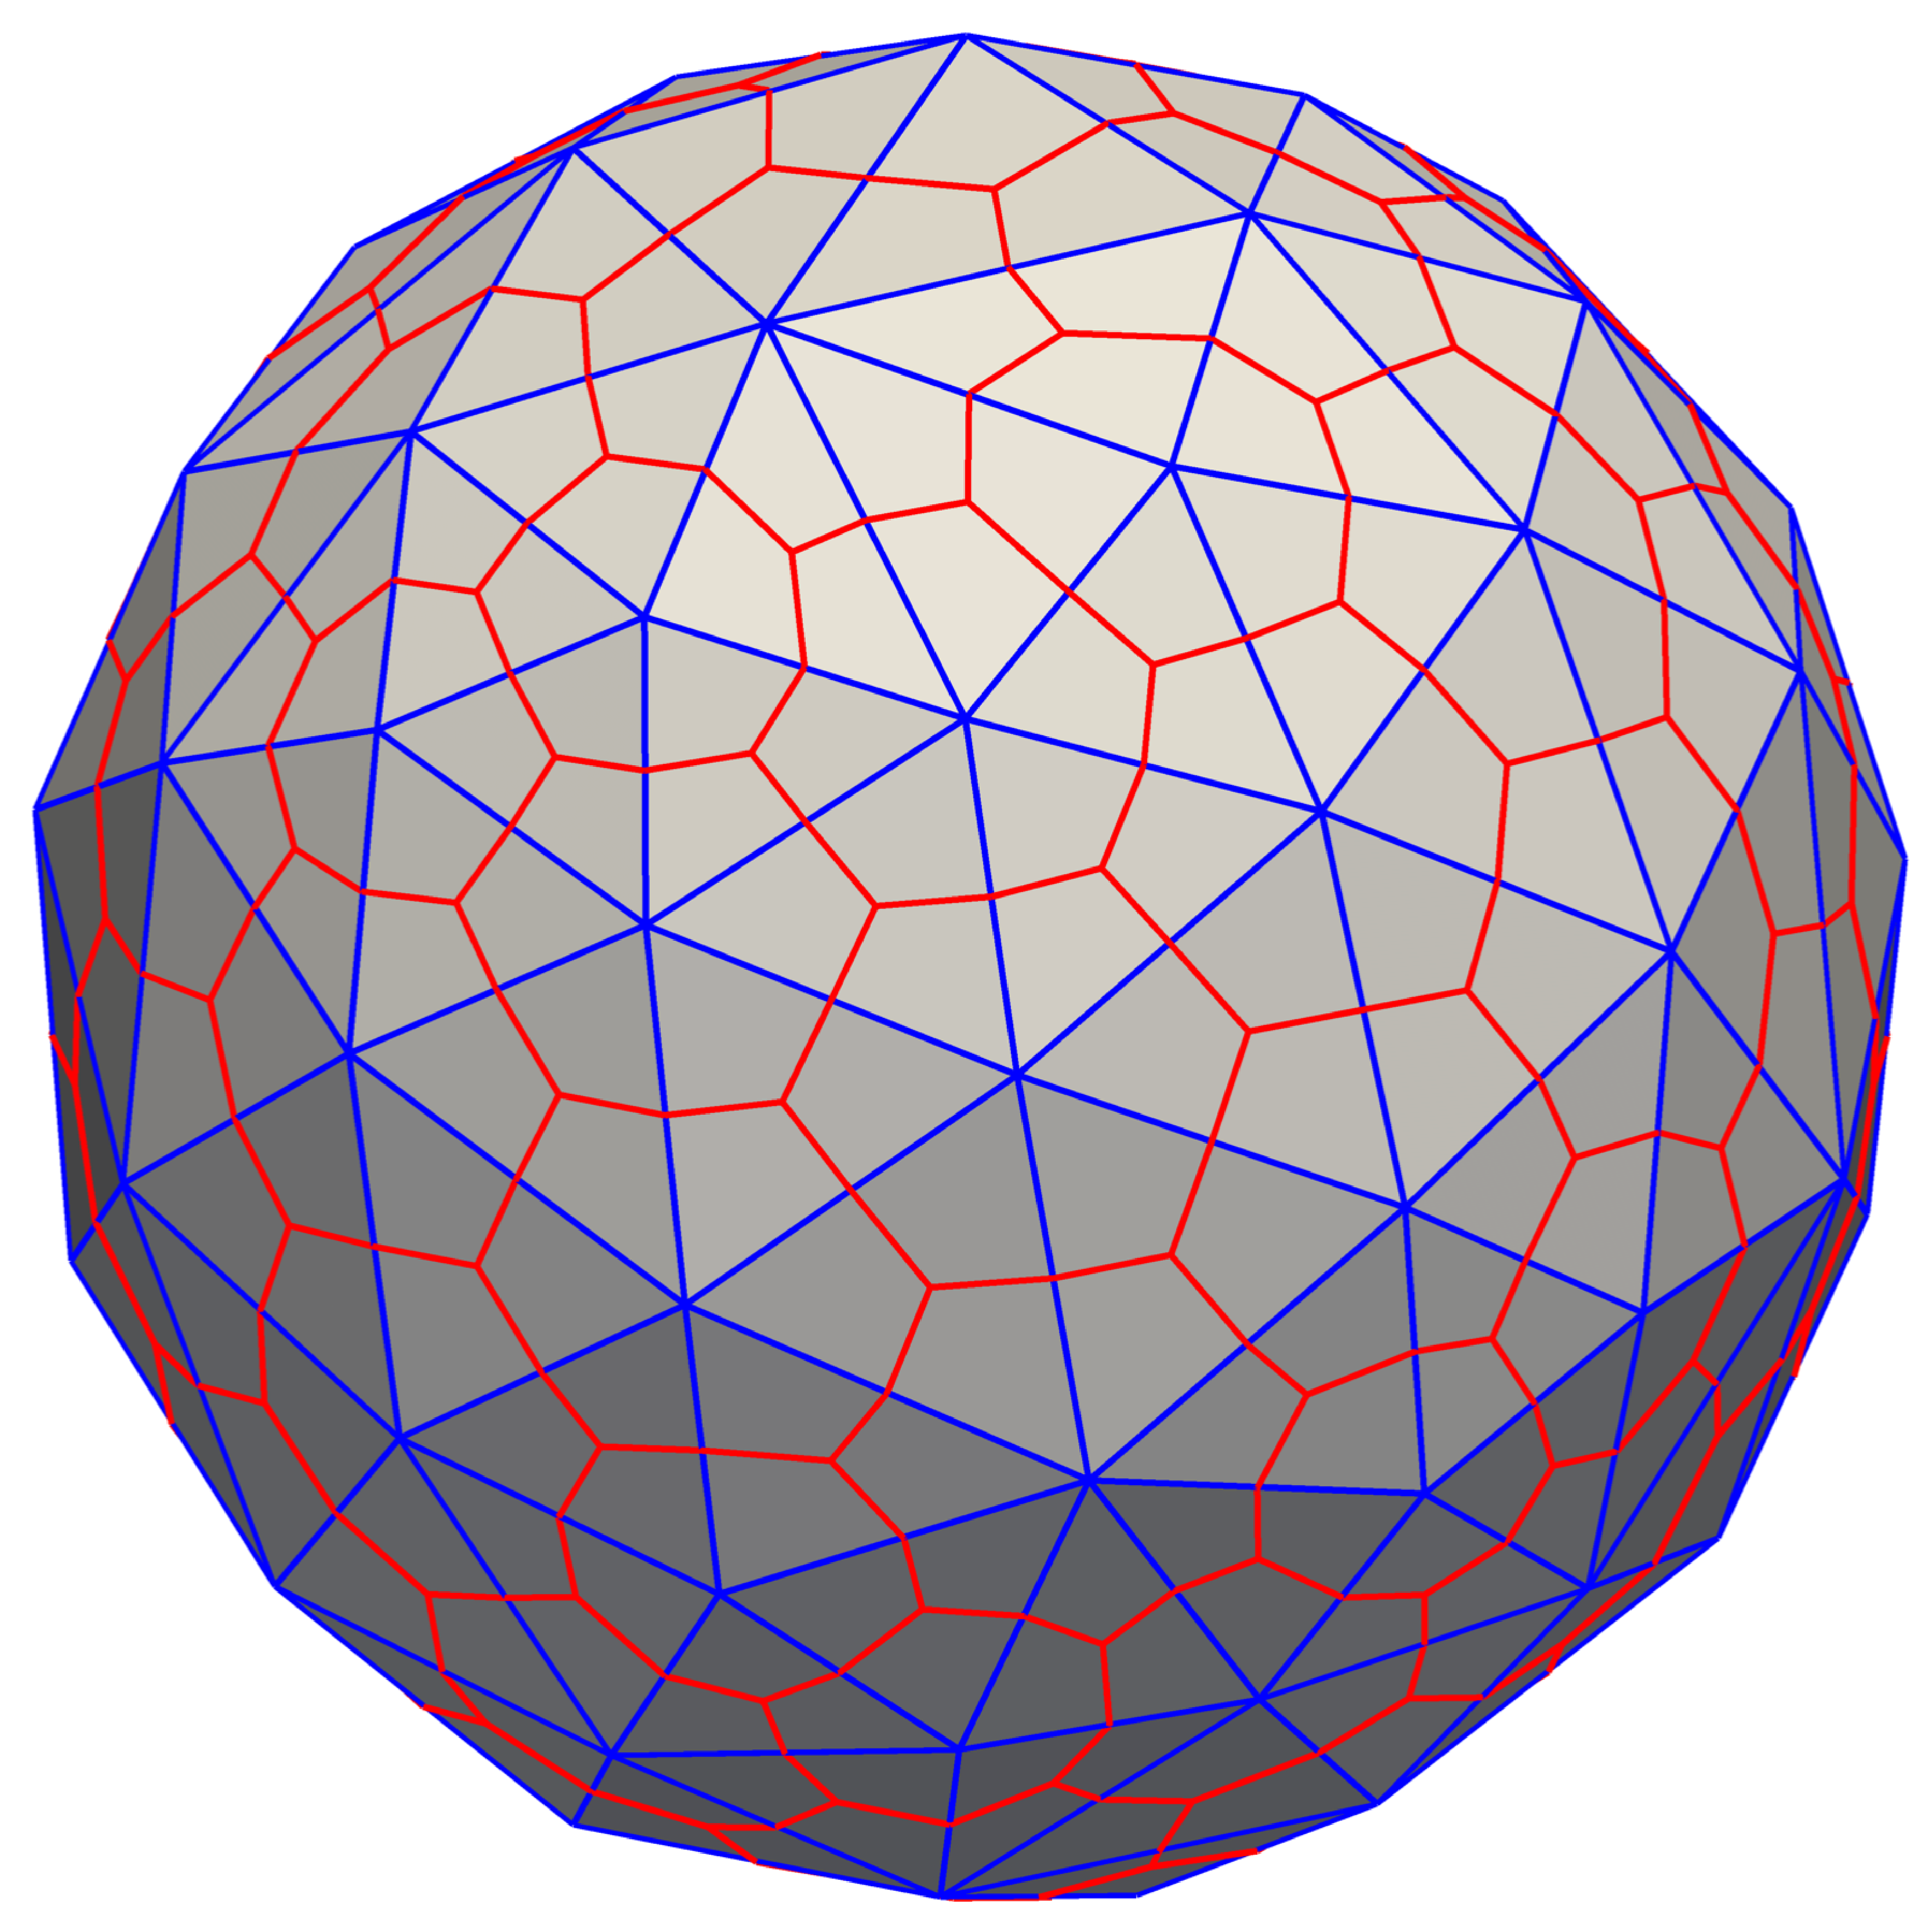
\includegraphics[width=0.6\textwidth]{img/sphere_primal_dual.pdf}};
\node[visible on=<3>] (plat) at (0,0) {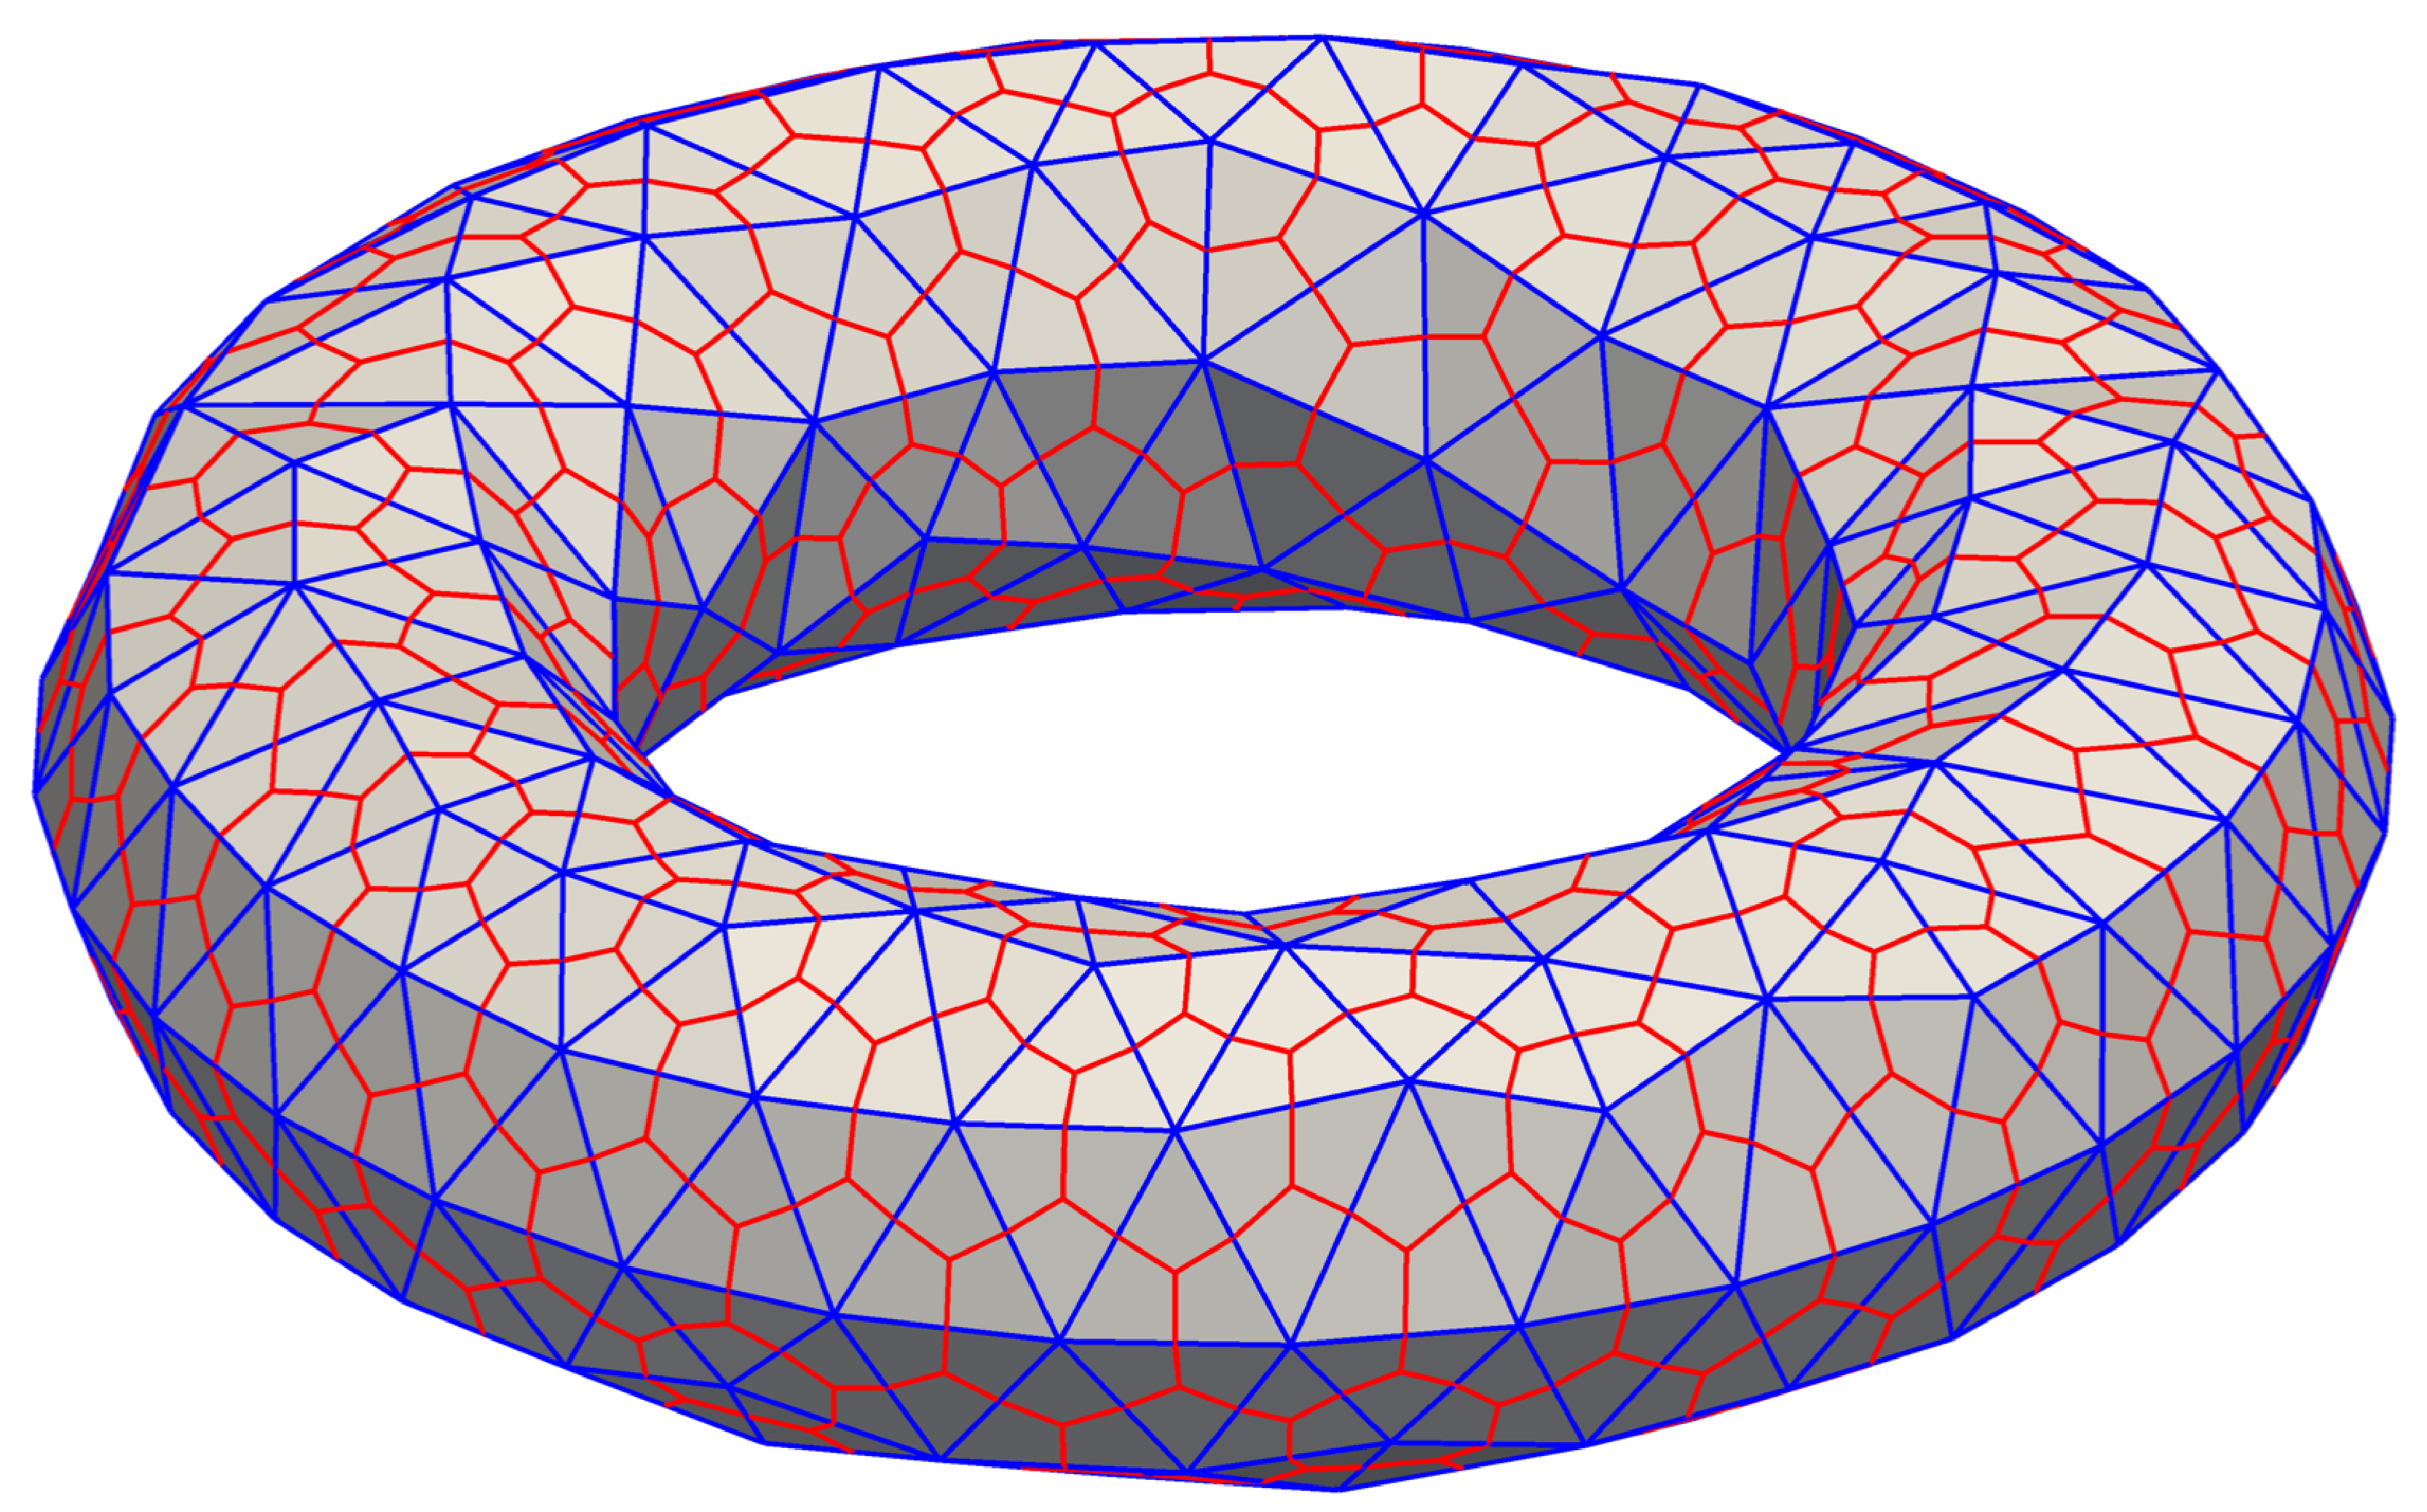
\includegraphics[width=0.7\textwidth]{img/torus_primal_dual.pdf}};
\node[visible on=<4->] (plat) at (0,0) {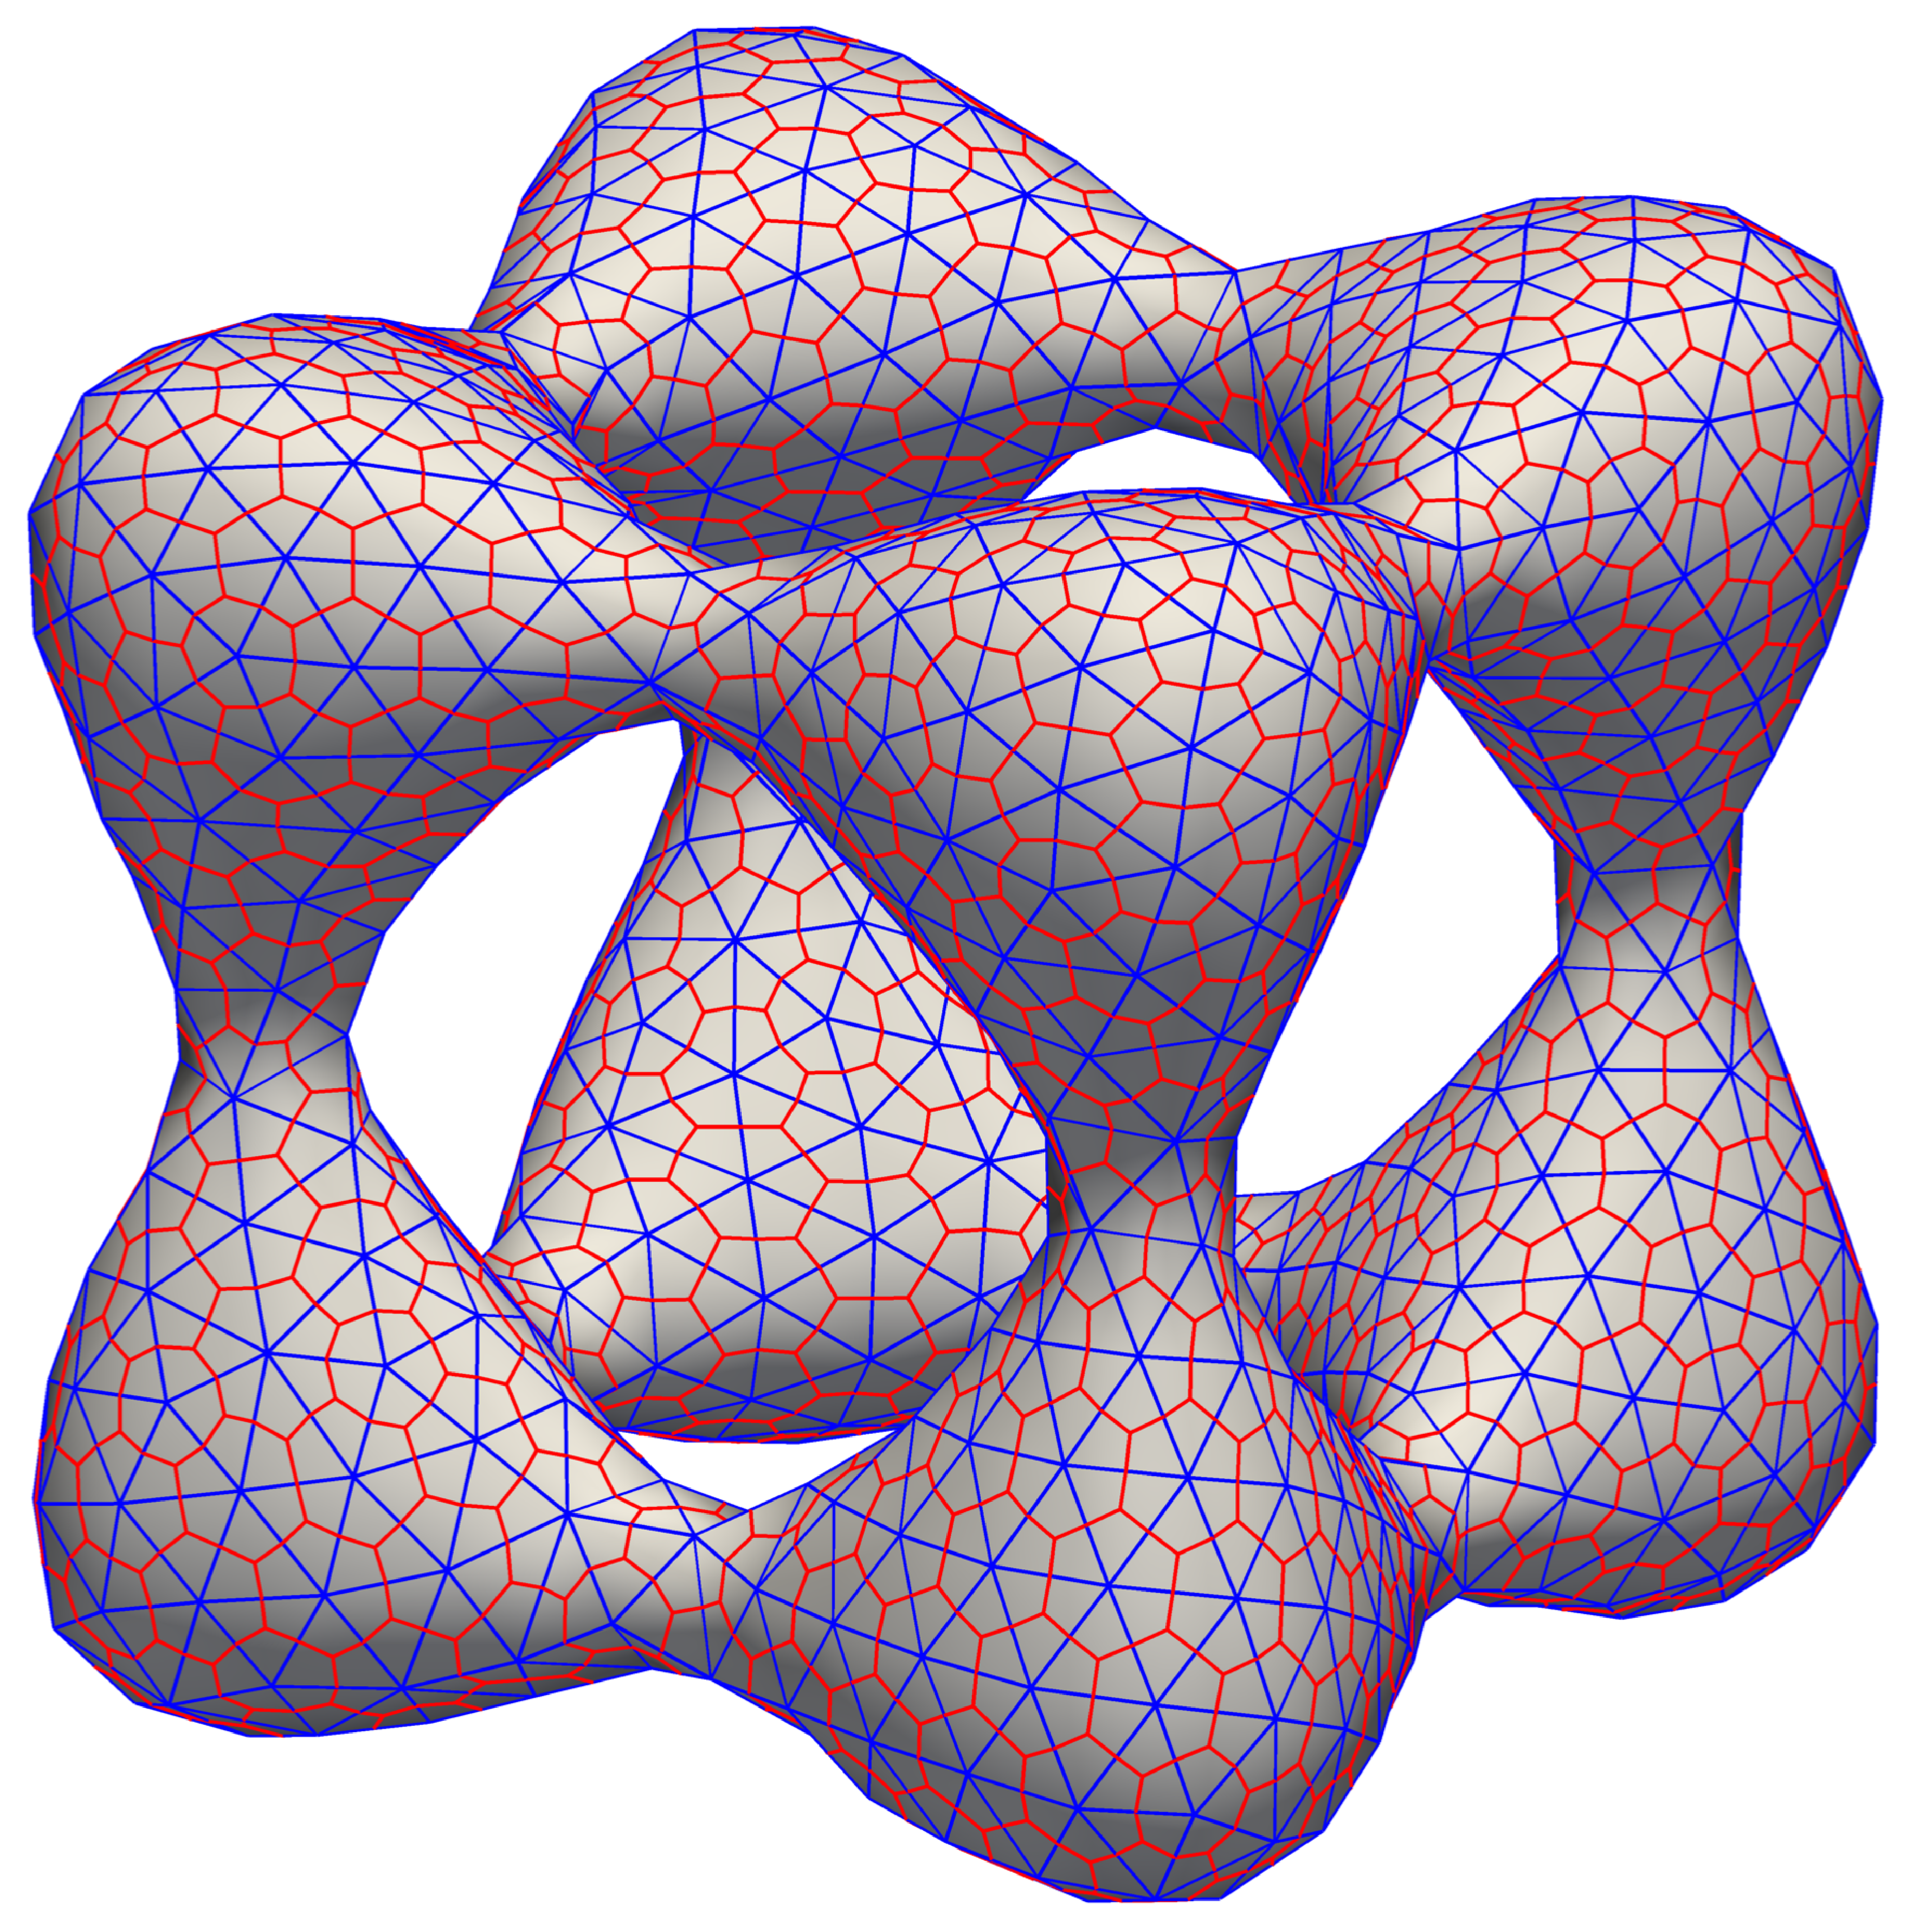
\includegraphics[width=0.6\textwidth]{img/tanglecube_primal_dual.pdf}};

\node[myblue, above left, text depth=0.25ex] at (plat.north) {primal $\ensprimalplat$};
\node[myred, above right, text depth=0.25ex, visible on=<2->] at (plat.north) {dual $\ensdualplat$};

\node[below] (sud) at (plat.south) {surface polyédrique};
\node[below] at (sud.south) {
    $
    \surfpoly = \displaystyle\bigcup_{\primalplat{K} \in {\color{myblue}\ensprimalplat}} {\color{myblue}\primalplat{K}}
    \onslide<2->{= \displaystyle\bigcup_{\mailledualeplate{K} \in {\color{myred}\ensdualplat}} {\color{myred}\mailledualeplate{K}}}
    $
    };

\end{tikzpicture}
